\documentclass{article}

\usepackage{graphicx}
\usepackage{tikz}
\usepackage{tikzsymbols}
\usetikzlibrary{calc,patterns,shapes.geometric}
\pagestyle{empty}
\usepackage[margin=0pt]{geometry}
\geometry{papersize={14in,12in}}

\def\centerarc[#1](#2)(#3:#4:#5){\draw[#1] ($(#2)+({#5*cos(#3)},{#5*sin(#3)})$) arc (#3:#4:#5);}

\begin{document}
	\begin{figure}
		\centering
		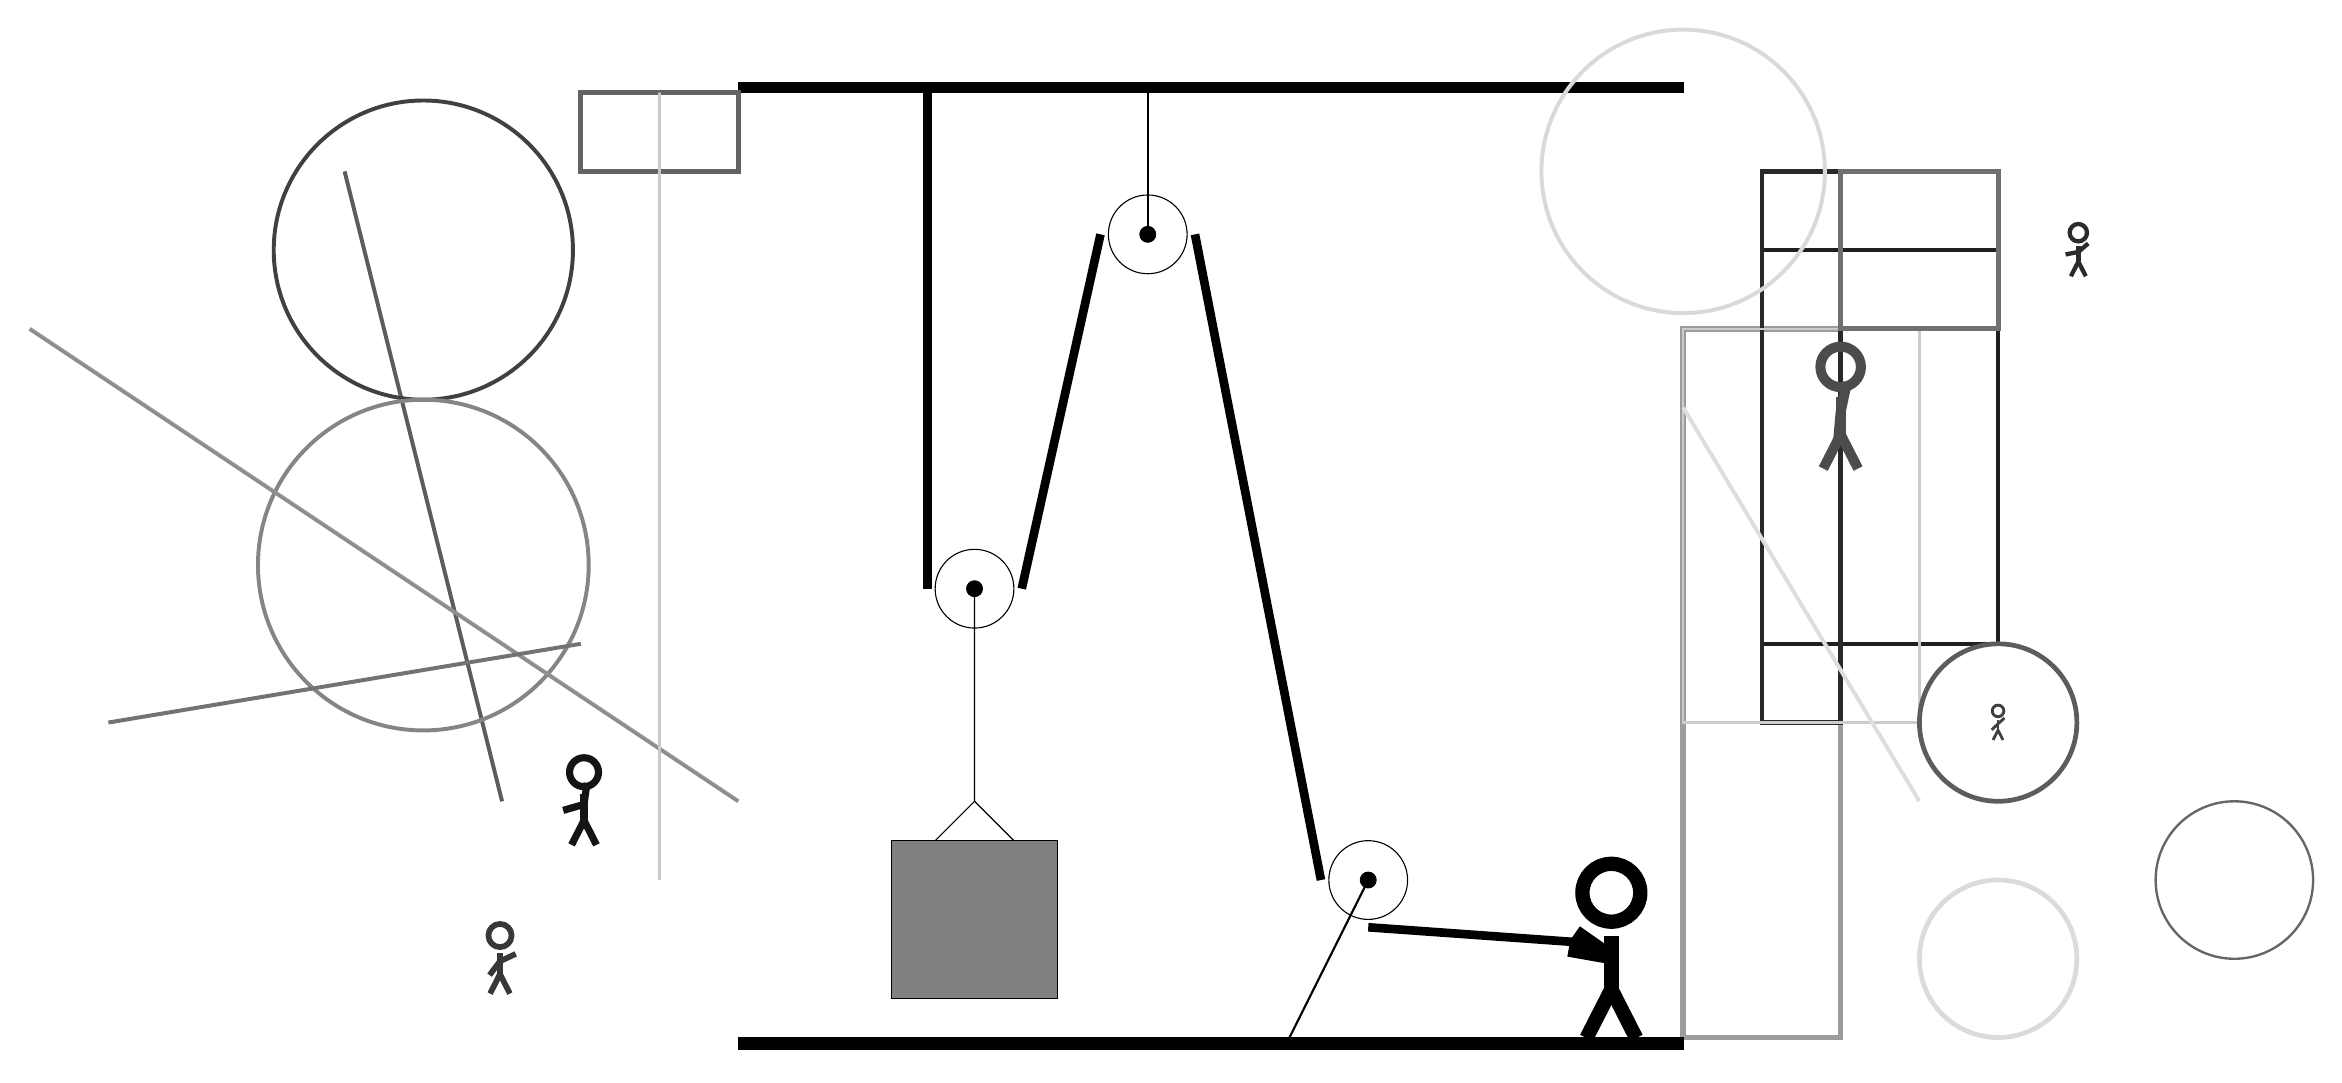
\begin{tikzpicture}
			%%%%% START %%%%%
			
			\draw[fill=black] (-2, 9) rectangle (10, 9.125);
			
			\draw (3.2, 7.2) circle (0.5);
			\draw[fill=black] (3.2, 7.2) circle (0.1);
			\draw[thick] (3.2, 7.2) -- (3.2, 9);
			
			\node[line width=0.7mm, color=black!75] at (14, 1) {\Strichmaxerl[2][44][42]};
			
			\draw[line width=0.5mm, color=black!64](-7, 8) -- (-5, 0);
			\node[line width=0.7mm, color=black!78] at (-5, -2) {\Strichmaxerl[4][53][25]};
			\draw[line width=0.7mm, color=black!39] (10, 6) rectangle (12, -3);
			\draw[line width=0.6mm, color=black!61] (-4, 8) rectangle (-2, 9);
			\draw[line width=0.5mm, color=black!88] (11, 7) rectangle (14, 2);
			\draw [line width=0.5mm, color=black!75](-6, 7) circle (1.9);
			\draw[line width=0.6mm, color=black!84] (12, 8) rectangle (11, 1);
			\draw[line width=0.3mm, color=black!20] (10, 6) rectangle (13, 1);
			
			\draw[line width=0.5mm, color=black!13](13, 0) -- (10, 5);
			\draw [line width=0.5mm, color=black!48](-6, 3) circle (2.1);
			\draw[line width=0.5mm, color=black!44](-2, 0) -- (-11, 6);
			\node[line width=0.6mm, color=black!83] at (15, 7) {\Strichmaxerl[3][11][41]};
			\draw [line width=0.6mm, color=black!64](14, 1) circle (1.0);
			\draw [line width=0.5mm, color=black!15](10, 8) circle (1.8);
			\node[line width=0.4mm, color=black!92] at (-4, 0) {\Strichmaxerl[5][16][82]};
			
			\draw[line width=0.5mm, color=black!55](-4, 2) -- (-10, 1);
			\draw [line width=0.6mm, color=black!14](14, -2) circle (1.0);
			\node[line width=0.3mm, color=black!70] at (12, 5) {\Strichmaxerl[7][85][78]};
			\draw[line width=0.4mm, color=black!21] (-3, -1) rectangle (-3, 9);
			\draw[line width=0.6mm, color=black!56] (12, 8) rectangle (14, 6);
			
			\draw [line width=0.3mm, color=black!60](17, -1) circle (1.0);
			
			
			\draw (6, -1) circle (0.5);
			\draw[fill=black] (6, -1) circle (0.1);
			\draw[thick] (6, -1) -- (5, -3);
			
			\draw (1, 2.7) circle (0.5);
			\draw[fill=black] (1, 2.7) circle (0.1);
			
			\draw (1, 2.7) -- (1, 0) -- (0.5, -0.5);
			\draw (1, 0) -- (1.5, -0.5);
			\draw[fill=black!50] (-0.05, -0.5) rectangle (2.05, -2.5);
			
			\draw[line width=1.1mm] (0.4, 9) -- (0.4, 2.7);
			\centerarc[line width=1.1mm](1, 2.7)(180:360:0.6);
			\draw[line width=1.1mm](1.6, 2.7) -- (2.6, 7.2);
			\centerarc[line width=1.1mm](3.2, 7.2)(0:180:0.6);
			\draw[line width=1.1mm](3.8, 7.2) -- (5.4, -1);
			\centerarc[line width=1.1mm](6, -1)(180:270:0.6);
			\draw[line width=1.1mm](6, -1.6) -- (8.8, -1.8);
			
			\node at (9, -1.9) {\Strichmaxerl[10][-35][170]};
			
			\draw[fill=black] (-2, -3) rectangle (10, -3.15);
			
			%%%%% END %%%%%
		\end{tikzpicture}
	\end{figure}	
\end{document}